\documentclass[
	classe=$2^{de}$
	headerTitle=Déplacements\space dans\space une\space ville
]{exercice}

\usepackage{tikz-repère}
\usepackage{tcolorbox}

\begin{document}

\begin{center}
	\includegraphics[width=\textwidth]{ville.png}
\end{center}

% \begin{tcolorbox}
% 	On dispose d'un plan de la ville, indiqué ci-dessus. Il vous faudra donner des instructions à votre camarade afin de se rendre à un point précis.

% 	Vous devez pour cela donner des instructions à votre binôme, de la forme «déplace-toi de ... mètres vers l'est, puis de ... mètres vers le nord», etc.
% \end{tcolorbox}

Voici le plan d'une ville : on se trouve sur le point \textbf{Départ}, et on va tenter d'atteindre les autres points.

\newcommand{\spacing}{3.5em}
\begin{enumerate}
	\item Décrire une série de mouvements de la forme «se déplacer de ... mètres vers l'est, puis de ... mètres vers le nord» qui permette d'atteindre le point \textbf{A}. \vspace{\spacing}
	\item De même, décrire une série de mouvements permettant d'atteindre le point \textbf{B}. \vspace{\spacing}
	\item Décrire maintenant une série de mouvements permettant d'atteindre le point de départ en \uline{partant de \textbf{C}}. \vspace{\spacing}
	\item Le point \textbf{D} est une personne, qui se déplace \uline{deux fois moins vite} que nous vers l'est. En partant vers le nord, allons-nous la croiser ? Justifier. \vspace{\spacing}
	\item Pour chacun des points \textbf{A}, \textbf{B} et \textbf{C}, décrire la série de mouvement à faire pour les atteindre depuis le point de départ, si on est à vol d'oiseau (c'est-à-dire si on peut passer au dessus des bâtiments). \vspace{\spacing}
\end{enumerate}

\end{document}